\chapter{Additional Index Structures}
\label{chap:additional-structures}
\vspace{-0.75cm}
\centerline{\rule{149mm}{.02in}}
\vspace{0.75cm}

This section describes index structures which were implemented during the project, but were not discussed or evaluated in the main report due to time constraints. Preliminary findings on the structures' performance is discussed.

\section{Multigrid Tree}
\label{sec:multigrid}

The Multigrid Tree decomposes the data space into a uniform grid by cutting each dimension into $B$ intervals. A cell is defined by the intervals of each dimension it is contained in. Formally, a cell is defined as a $d - 1$ tuple  $C = \lbrace c_0, c_1, \dots, c_{d - 1} \rbrace$, where	 $c_i$ is the interval the cell belongs to in dimension $i$. There are a total of $B^d$ cells. Figure \ref{fig:multigrid-decomposition} illustrates how the Multigrid Tree decomposes 2D data space when $B = 8$, resulting in $8^2 = 64$ cells. Each cell corresponds to a bucket in the Multigrid Tree.

This structure is a hybrid of hash-based and tree-based structures. It is a tree where each leaf node is a bucket containing one or more points and non-leaves are hash tables. Each non-leaf hashes points to the interval the point is contained in, for a single dimension $i$. The bucket a point is hashed to is another node of the Multigrid Tree. This node is either another hash table, which hashes points based on which interval of dimension $i + 1$ they are inside, or a bucket (i.e. an array of points).

The root node always hashes points using the interval of dimension 0 they are contained in. When these buckets exceed a certain capacity, say $M$, then the bucket is turned into a hash table which hash points to their interval in dimension 1. This is repeated until the last dimension, $d - 1$, is reached. At this point, there are no more dimensions to discriminate points with, so the buckets are not transformed into hash tables when their size exceeds $M$. 

In effect, this creates a tree where the maximum height is $d + 1$ and each non-leaf node has at most $B$ children that correspond to the $B$ intervals of the dimension it is discriminating against. All non-leaf nodes at level $i$ of the tree hash points to the interval of dimension $i$ they belong to. The hashing function for dimension $i$ is given below:

\begin{equation}
	h_i(p) = \floor*{\frac{p_i - min_i}{max_i - min_i} \times B}
	\label{eq:multigrid-hash}
\end{equation}
where $p$ is a point and $min_i, max_i$ are the lower and upper boundaries of dimension $i$.

Figure \ref{fig:multigrid-root} shows a Multigrid Tree with a single non-leaf node and its accompanying spatial decomposition in 2D. Notice how points are discriminated only using the value of the $x$ dimension. Figure \ref{fig:multigrid-multiple-levels} shows a Multigrid Tree where some of the bucket sizes have exceeded $M$, which is 3 in this case. Notice how some intervals in the $x$ dimension have been sliced in the $y$ dimension now, allowing for greater discrimination.

Equation \ref{eq:multigrid-hash} can clearly be computed in constant time. Since there are at most $d + 1$ levels in the tree, at most $d$ instances of Equation \ref{eq:multigrid-hash} will be computed. It follows that retrieving the bucket a point is contained in takes $O(d)$ time. If points are uniformly distributed across the grid, then this structure will take $O(d)$ time for all operations.  However, it is possible for all the points in a dataset to be mapped to the same cell, making \texttt{insert}, \texttt{delete} and point queries take $O(n)$ time.

For highly skewed datasets, most of the points will end up being mapped to the same few cells. This causes the structure to degenerate to Sequential Scan in a similar manner to the Pyramid Tree (see Section \ref{sec:implications-to-md-search}). Figure \ref{fig:multigrid-clustered} illustrates this limitation. Despite both dimensions being used to discriminate between points, they are all get hashed to the same value because they are contained in the same cell.

\begin{figure}
	\begin{center}
		\begin{subfloat}[Full Multigrid Tree Decomposition\label{fig:multigrid-decomposition}]{%
			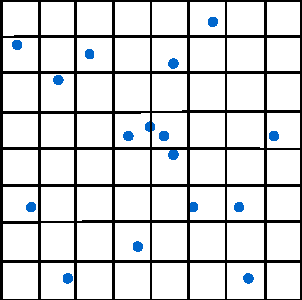
\includegraphics[scale=0.65]{figures/multigrid_decomposition.pdf}
		}
		\end{subfloat}~~~~~
		\begin{subfloat}[t][Multigrid Tree Decomposition with Clustered Data\label{fig:multigrid-clustered}]{%
			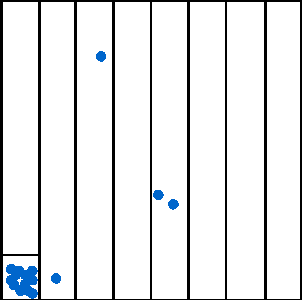
\includegraphics[scale=0.65]{figures/multigrid_clustered.pdf}
		}
		\end{subfloat}
	\end{center}

	\caption{Multigrid Tree Decompositions}
	\label{fig:multigrid-decompositions}
\end{figure}

\begin{figure}
	\begin{center}
		\begin{subfloat}[Multigrid Tree with Minimum Height\label{fig:multigrid-root}]{%
			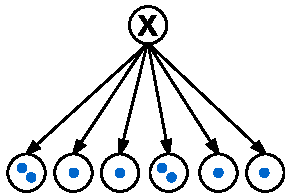
\includegraphics[scale=0.65]{figures/multigrid_root_tree.pdf}
			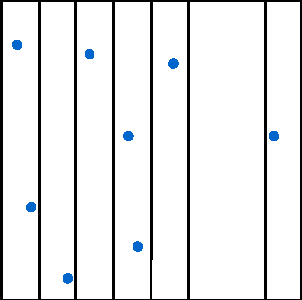
\includegraphics[scale=0.65]{figures/multigrid_root.pdf}
		}
		\end{subfloat}~~~~~
		\begin{subfloat}[Multigrid Tree with Maximum Height\label{fig:multigrid-multiple-levels}]{%
			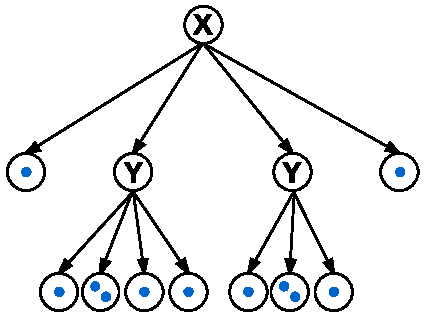
\includegraphics[scale=0.65]{figures/multigrid_levels_tree.pdf}
			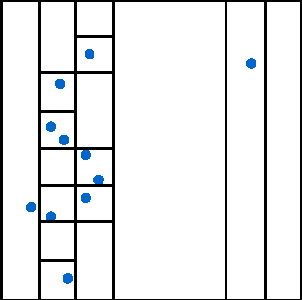
\includegraphics[scale=0.65]{figures/multigrid_levels.pdf}
		}
		\end{subfloat}
	\end{center}

	\caption{Multigrid Trees and their Respective Spatial Decompositions in 2D}
	\label{fig:multigrid-trees}
\end{figure}

\section{iMinMax($\theta$)}

iMinMax($\theta$) is an index structure similar to the Pyramid Tree, whose behaviour is affected by the parameter $\theta$ \cite{iminmax}. $\theta$ can be tuned to optimise the structure for different data distributions. Like the Pyramid Tree, it reduces points to a single dimension and applies a one-dimensional index structure to these values. To dynamically adapt the spatial decomposition to different point distributions, the value of $\theta$ is tweaked. This changes the hashing function, meaning the structure must be rebuilt every time $\theta$ is changed.

An implementation of this was developed using the base hash structure described in Section \ref{sec:bucket-hash-structure}. Preliminary tests revealed that the structure was only slightly faster than the Pyramid Tree for the astrophysics and hurricane Isabel datasets, regardless of which value was chosen for $\theta$. The majority of the structure's execution time was spent rebuilding the structure, supporting the claim that existing dimension reduction techniques will require rebuilding are not suitable for dynamic data (discussed in Section \ref{sec:implications-to-md-search}).

\section{Bucket $kd$-Tree}

Instead of storing a single point in every node of the tree, the Bucket $kd$-Tree stores multiple points in each node (termed a bucket), with the constraint that only leaf nodes store points. Non-leaf nodes serve to partition the data space, each cutting the space along a single dimension by some value (the cutting value). When the number of points in a leaf exceeds a certain number, say $M$, then a cutting dimension and value are determined, which are used to split a leaf into two. The left and right children nodes are leaves that contain the points from the split node that lie on each side of the split.

To query or delete a point, the leaf containing the point is found, which is sequentially scanned to find the point. If the point is found, it is removed from the leaf. If the total number of points being stored in the modified leaf node and its sibling is less than $\frac{M}{4}$, then the two leaf nodes are \textit{merged} into their parent. The parent becomes a leaf node containing all the points stored in the two leaves.

Compared to the point $kd$-tree, the bucket $kd$-tree has more knowledge about the data's distribution since multiple points are stored in a bucket. With the point $kd$-tree, only one point at a time is used to determine the cutting dimension, so less knowledge about the distribution is used to perform a split. Knowing more about the distribution allows the bucket $kd$-tree to partition the data more effectively to construct a more balanced tree.

This structure was implemented as part of the project. The \textit{sliding midpoint} splitting rule was used to split full leaves, which is described in \cite{sliding-midpoint-split}. Preliminary results show that it reduced balance factor, but an inefficient implementation meant there were large constant factors that made the structure slower than the point $kd$-tree implementation. More work optimising the implementation should be performed to assess its suitability for dynamic scientific datasets.